%!TEX root = ../main.tex
\documentclass{beamer} % Gliederung im Kopf, sections und subsections
\renewcommand{\baselinestretch}{1.2}\normalsize
\usetheme{default}
\setbeamertemplate{navigation symbols}{}
\setbeamertemplate{footline}[frame number]

\usepackage{tabu}
\usepackage{etex}
%\usepackage{beamerthemesplit}
%\useoutertheme[subsection=false]{smoothbars}
%\usepackage[final]{pdfpages}
\usepackage{bibentry}
\usepackage{bm}
\usepackage{bigints}
\usepackage{graphicx}
\usepackage{relsize}
\usepackage[round,longnamesfirst]{natbib}
\usepackage{bm}																									%matrix symbol
\usepackage{bbm}

\usepackage{paralist}

\usepackage{algpseudocode}
\usepackage{algorithmicx}
\usepackage{verbatim}
\usepackage{setspace}																					%Fu�noten (allgm.
\usepackage{hyperref}

\usepackage{bibentry}

\DeclareMathOperator*{\argmin}{arg\,min}
\DeclareMathOperator*{\argmax}{arg\,max}

\nobibliography*
\renewcommand{\vec}[1]{\mathbf{#1}}

\hypersetup{colorlinks=true,urlcolor=blue}														%Zeilenabst�nde)
\usepackage{threeparttable}
\usepackage{subfig}
\usepackage{epstopdf}
\usepackage{lscape}																							%Querformat
\usepackage[latin1]{inputenc}																		%Umlaute
\usepackage{graphicx}
\graphicspath{{../../material/}}

\usepackage{booktabs}
\usepackage{amsmath}
\usepackage{amssymb}
%\usepackage{uarial}

\usepackage{tabularx}
\usepackage{fancybox}																						%Boxen und Rahmen
\usepackage{appendix}
\usepackage{enumerate}

%EURO Symbol
\usepackage{tabularx}
\usepackage{longtable}																					%Mehrseitige Tabellen
\usepackage{fix-cm}
\usepackage[T1]{fontenc}
\usepackage{color,colortbl}																			%Farbige Tabellen
\usepackage{threeparttable}
\usepackage{hyperref}
\usepackage{amsfonts}

\usepackage{graphicx}
\usepackage{caption}

\usepackage{tikz}
\tikzset{
  treenode/.style = {shape=rectangle, rounded corners,
                     draw, align=center,
                     top color=white, bottom color=blue!20},
  root/.style     = {treenode, font=\Large, bottom color=red!30},
  env/.style      = {treenode, font=\ttfamily\normalsize},
  dummy/.style    = {circle,draw}
}
%\usepackage{cmbright}
\def\newblock{\hskip .11em plus .33em minus .07em}
\newcommand{\bs}{\boldsymbol}
\newcommand{\N}{\mathbb{N}}
\newcommand{\cov}{\mathrm{cov}\thin}
\newcommand{\thin}{\thinspace}
\newcommand{\thick}{\thickspace}

\newcommand{\vect}[1]{\mathbf{#1}}
\newcommand{\myfrac}[3][0pt]{\genfrac{}{}{}{}{\raisebox{#1}{$#2$}}{\raisebox{-#1}{$#3$}}}
\newcommand{\U}{\mathrm{U}}	%Uniform Distribution
\newcommand{\D}{\mathrm{D}}	%Dirichlet Distribution
\newcommand{\W}{\mathrm{W}}	%Wishart Distribution
\newcommand{\E}{\mathrm{E}}		%Expectation
\newcommand{\Prob}{\mbox{Pr}}		%Expectation
\newcommand{\Iden}{\mathbb{I}}	%Identity Matrix
\newcommand{\Ind}{\mathrm{I}}	%Indicator Function
\newcommand{\Tau}{\mathcal{T}\thin}

\newcommand{\var}{\mathrm{var}\thin}
\newcommand{\plim}{\mathrm{plim}\thin}
\newcommand\indep{\protect\mathpalette{\protect\independenT}{\perp}}
\def\independenT#1#2{\mathrel{\rlap{$#1#2$}\mkern5mu{#1#2}}}
\newcommand{\notindep}{\ensuremath{\perp\!\!\!\!\!\!\diagup\!\!\!\!\!\!\perp}}%

\newcommand{\mc}{\multicolumn}

\newcommand{\ph}{\phantom}
% weitere Optionen:
% secbar: Gliederung im Kopf, nur sections (alternativ zu subsecbar)
% handout: Produktion von Handouts, keine Animationen
\definecolor{darkblue}{rgb}{0,.35,.62}
\definecolor{lightblue}{rgb}{0.8,0.85,1}
\definecolor{lightgrey}{gray}{0.1}	%Farben mischen

%	kbordermatrix options

\makeatletter
\newcommand{\vast}{\bBigg@{4}}
\newcommand{\Vast}{\bBigg@{5}}
\makeatother
\newcommand{\indicator}[1]{\mathbbm{1}{\left\{ {#1} \right\} }}
\newcommand{\indic}{1{\hskip -2.5 pt}\hbox{1} }


\definecolor{lightgrey}{gray}{0.90}	%Farben mischen
\definecolor{grey}{gray}{0.85}
\definecolor{darkgrey}{gray}{0.65}
\definecolor{lightblue}{rgb}{0.8,0.85,1}

\renewcommand{\arraystretch}{1.5}


\usepackage{tikz}
\usetikzlibrary{trees,shapes,arrows,decorations.pathmorphing,backgrounds,positioning,fit,petri}
\renewcommand*{\familydefault}{\sfdefault}

\tikzset{forestyle/.style = {rectangle, thick, minimum width = 5cm, minimum height = 0.5cm, text width = 4.5cm, outer sep = 1mm},
	pre/.style={<-, shorten <=1pt, >=stealth, ultra thick},
	extend/.style={<-,dashed, shorten <=1pt, >=stealth, ultra thick}}
\captionsetup[subfigure]{labelformat=empty}


\newcommand{\beginbackup}{
   \newcounter{framenumbervorappendix}
   \setcounter{framenumbervorappendix}{\value{framenumber}}
}
\newcommand{\backupend}{
   \addtocounter{framenumbervorappendix}{-\value{framenumber}}
   \addtocounter{framenumber}{\value{framenumbervorappendix}}
}


% Begin Full Justification ---------------------------------------------------------

\usepackage{ragged2e}
% \usepackage{etoolbox}
\usepackage{lipsum}
\makeatletter
\renewcommand{\itemize}[1][]{%
  \beamer@ifempty{#1}{}{\def\beamer@defaultospec{#1}}%
  \ifnum \@itemdepth >2\relax\@toodeep\else
    \advance\@itemdepth\@ne
    \beamer@computepref\@itemdepth% sets \beameritemnestingprefix
    \usebeamerfont{itemize/enumerate \beameritemnestingprefix body}%
    \usebeamercolor[fg]{itemize/enumerate \beameritemnestingprefix body}%
    \usebeamertemplate{itemize/enumerate \beameritemnestingprefix body begin}%
    \list
      {\usebeamertemplate{itemize \beameritemnestingprefix item}}
      {\def\makelabel##1{%
          {%
            \hss\llap{{%
                \usebeamerfont*{itemize \beameritemnestingprefix item}%
                \usebeamercolor[fg]{itemize \beameritemnestingprefix item}##1}}%
          }%
        }%
      }
  \fi%
  \beamer@cramped%
  \justifying% NEW
  %\raggedright% ORIGINAL
  \beamer@firstlineitemizeunskip%
}

\justifying

% \apptocmd{\frame}{\justifying}{}{}

\usepackage{array}
\newcolumntype{L}[1]{>{\raggedright\let\newline\\\arraybackslash\hspace{0pt}}m{#1}}
\newcolumntype{C}[1]{>{\centering\let\newline\\\arraybackslash\hspace{0pt}}m{#1}}
\newcolumntype{R}[1]{>{\raggedleft\let\newline\\\arraybackslash\hspace{0pt}}m{#1}}



% End Full Justification ------------------------------------------------------------


\title{Parameters of Interest}
\author{Philipp Eisenhauer}

\date{}

\let\otp\titlepage
%\renewcommand{\titlepage}{\otp\addtocounter{framenumber}{-1}}

\begin{document}
\maketitle

%-------------------------------------------------------------------------------
%-------------------------------------------------------------------------------
\begin{frame}\begin{center}
\LARGE\textit{Housekeeping}
\end{center}\end{frame}
%-------------------------------------------------------------------------------
%-------------------------------------------------------------------------------
\begin{frame}
Since nearly all of you choose to review experimental studies. Please be sure to read ...

\begin{itemize}
\item \bibentry{Deaton.2010}
\item \bibentry{Imbens.2009}
\item \bibentry{Heckman.2009t}
\end{itemize}
\end{frame}

\begin{frame}
\textbf{Student Presentation}
\begin{itemize}
\item 20 minutes of presentation and discussion
\item peer-review of presentation\vspace{0.5cm}
\end{itemize}

\textbf{Lectures}
\begin{itemize}
\item constantly updated and available at\vspace{0.2cm}
\begin{center}\url{https://github.com/policyMetrics/course/wiki}\end{center}
\end{itemize}
\end{frame}

\begin{frame}
\begin{figure}
\caption{Book Recommendations}
\subfloat[]{
\scalebox{0.3}{
\includegraphics{fig-academic-writing-1}}}\hspace{0.5cm}
\subfloat[]{
\scalebox{0.3}{
\includegraphics{fig-academic-writing-2}}}
\end{figure}
\end{frame}


\begin{frame}
\begin{figure}
\caption{Book Recommendations}
\subfloat[]{
\scalebox{0.3}{
\includegraphics{fig-academic-presentation-1}}}\hspace{0.5cm}
\subfloat[]{
\scalebox{0.3}{
\includegraphics{fig-academic-research-1}}}
\end{figure}
\end{frame}


\begin{frame}
We need to slightly modify the notation, and thus the economics, of our conceptual framework to better align it with the published work on the topic. In the future, we will be more agnostic about what the agents care about and what they know when making their treatment decision.
\end{frame}

\begin{frame}
\textbf{Earlier Version}

\begin{align*}\begin{array}{l@{\qquad}l}
\text{Potential Outcomes} & \text{Cost} \\
Y_1 = \mu_1(X) + U_1      &C = \mu_D(Z) + U_C \\
Y_0 = \mu_0(X) + U_0      & \\
    & \\
\text{Observed Outcomes } & \text{Choice} \\
Y = D Y_1 + (1 - D)Y_0 & S = Y_1 - Y_0 - C \\
                       & D = \mathrm{I}[S > 0] \\
\end{array}\end{align*}
\end{frame}


\begin{frame}
\textbf{The Generalized Roy Model}

\begin{align*}\begin{array}{l@{\qquad}l}
\text{Potential Outcomes} &\text{Observed Outcome}\\
Y_1 = \mu_1(X) + U_1      &  Y = D Y_1 + (1 - D)Y_0 \\
Y_0 = \mu_0(X) + U_0      &\\
    & \\
\text{Choice} & \\
D = \mathrm{I}[\mu_D(X, Z) - V > 0] & \\
\end{array}
\end{align*}
\end{frame}
%-------------------------------------------------------------------------------
%-------------------------------------------------------------------------------
\maketitle

\begin{frame}
\citet{Heckman.2008a} sets out three tasks for us:

\begin{itemize}
\item Defining the Set of Hypotheticals or Counterfactuals \\\hspace{0.3cm}
    $\Rightarrow$ A Scientific Theory
\item Identifying Causal Parameters from Real Data \\\hspace{0.3cm}
    $\Rightarrow$ Mathematical Analysis of  Data Point or Set Identification
\item Identifying Parameters from Real Data\\\vspace{0.3cm}\hspace{0.3cm}
    $\Rightarrow$ Estimation and Testing Theory
\end{itemize}

\end{frame}
%-------------------------------------------------------------------------------
%-------------------------------------------------------------------------------
\begin{frame}\begin{center}
\LARGE\textit{Setup}
\end{center}\end{frame}
%-------------------------------------------------------------------------------
%-------------------------------------------------------------------------------
\begin{frame}
\textbf{The Generalized Roy Model}

\begin{align*}\begin{array}{l@{\qquad}l}
\text{Potential Outcomes} &\text{Observed Outcome}\\
Y_1 = \mu_1(X) + U_1      &  Y = D Y_1 + (1 - D)Y_0 \\
Y_0 = \mu_0(X) + U_0      &\\
    & \\
\text{Choice} & \\
D = \mathrm{I}[\mu_D(X, Z) - V > 0] & \\
\end{array}
\end{align*}
\end{frame}

\begin{frame}
\textbf{Useful Notation}

\begin{align*}
P(X, Z) & = \Pr(D = 1\mid X, Z) = F_V(\mu_D(X, Z)) \\
U_D     & = F_V(V)
\end{align*}

\end{frame}

\begin{frame}\textbf{Specification}\vspace{0.3cm}

We follow the parameterization in \citet{Heckman.2005e}:

\begin{align*}\begin{array}{l@{\qquad}l@{\qquad}l@{\qquad}l}
Y_1 = \gamma + \alpha + U_1 & U_1 = \sigma_1 \epsilon & \gamma = 0.670          & \sigma_1 = \phantom{-}0.012 \\
Y_0 = \gamma + U_0          & U_0 = \sigma_0 \epsilon & \alpha = 0.200          & \sigma_0 = -0.050 \\
D = \mathrm{I}[Z - V > 0]   & V\phantom{_0} = \sigma_V \epsilon   & \epsilon \sim \N(0, 1) & \sigma_V = -1.000 \\
\end{array}\end{align*}

\begin{align*}\begin{array}{l@{\qquad}l}
Z \sim \N(-0.0026, 0.2700)  & U_D = \Phi\left(\frac{V}{\sigma_V\sigma_\epsilon}\right)\\
\end{array}\end{align*}

\end{frame}
%-------------------------------------------------------------------------------
%-------------------------------------------------------------------------------
\begin{frame}\begin{center}
\LARGE\textit{Individual Heterogeneity}
\end{center}\end{frame}
%-------------------------------------------------------------------------------
%-------------------------------------------------------------------------------

\begin{frame}

Individual-specific Benefit of Treatment
\begin{align*}
Y_1 - Y_0 = (\mu_1(X) - \mu_0(X)) + (U_1 - U_0)\\
\end{align*}

\textbf{Sources of Heterogeneity}
\begin{itemize}
	\item Difference in Observable Characteristics
	\item Difference in Unobservable Characteristics
	\begin{itemize}
		\item  Uncertainty
		\item Private Information
	\end{itemize}
\end{itemize}
\end{frame}


\begin{frame}
\begin{figure}\caption{Distribution of Benefits}
\scalebox{0.35}{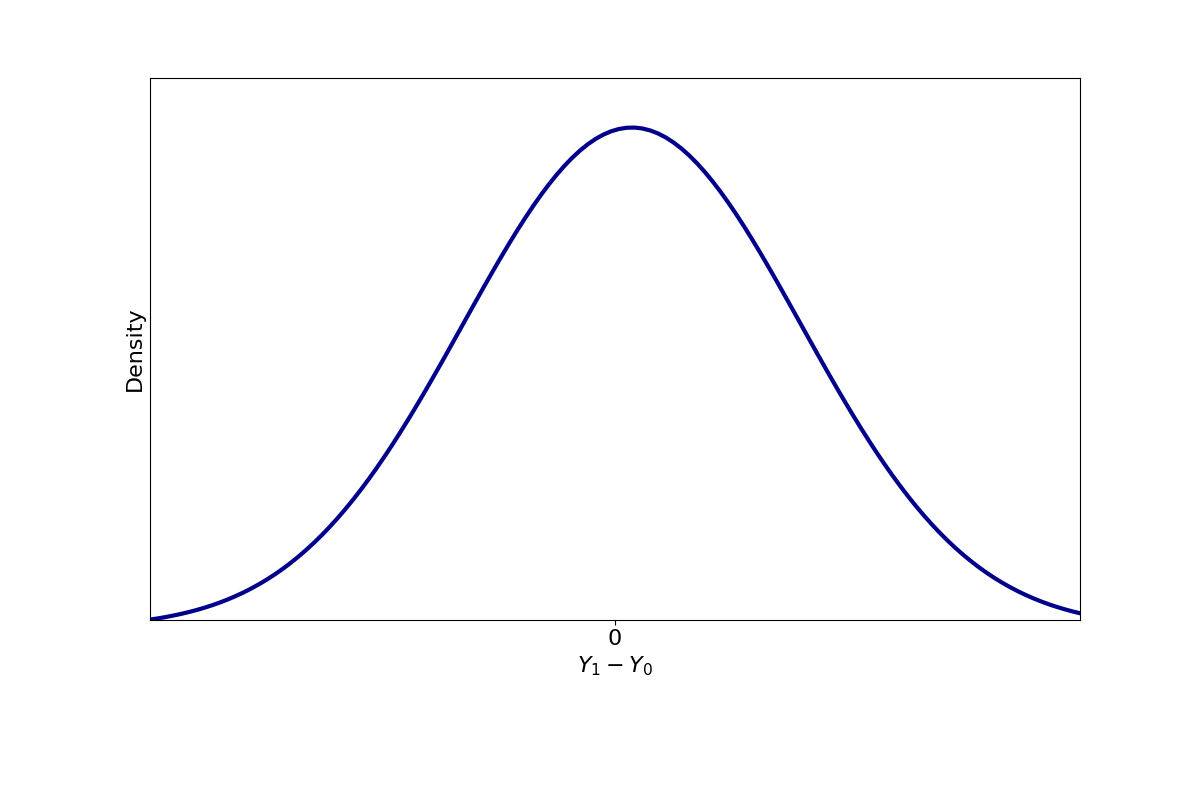
\includegraphics{fig-treatment-effects-benefits.png}}
\end{figure}
\end{frame}

\begin{frame}
\textbf{Essential Heterogeneity}\vspace{0.5cm}

\textbf{Definition:} Individuals select their treatment status based on
gains unobservable by the econometrician. More formally,

\begin{align*}
Y_1 - Y_0 \notindep D\quad \mid X = x.
\end{align*}

\(\Rightarrow\) consequences for the choice of the estimation strategy

\end{frame}


\begin{frame}
\begin{figure}\caption{Conditional Expectation and Essential Heterogeneity}
\scalebox{0.35}{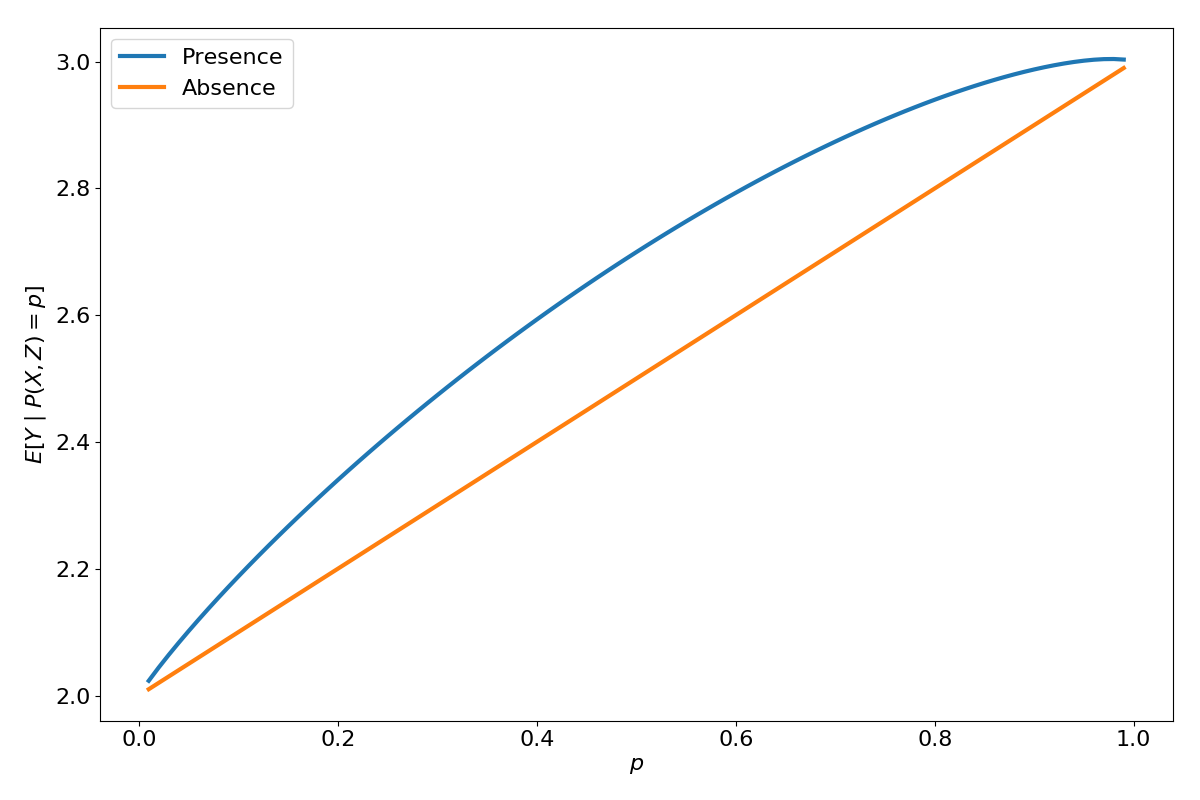
\includegraphics{fig-eh-conditional-expectation}}
\end{figure}
\end{frame}
%-------------------------------------------------------------------------------
%-------------------------------------------------------------------------------
\begin{frame}\begin{center}
\LARGE\textit{Conventional Average Treatment Effects}
\end{center}\end{frame}
%-------------------------------------------------------------------------------
%-------------------------------------------------------------------------------


\begin{frame}
\textbf{Conventional Average Treatment Effects}

\begin{align*}
B^{ATE} & = E[Y_1 - Y_0 ]\\
B^{TT} & = E[Y_1 - Y_0 \mid D = 1]\\
B^{TUT} & = E[Y_1 - Y_0 \mid D = 0]\\
\end{align*}

\(\Rightarrow\) correspond to \emph{extreme} policy alternatives

\end{frame}


\begin{frame}
\textbf{Selection Problem}

\begin{align*}
E[Y\mid D = 1] - E[Y\mid D = 0] & = \underbrace{E[Y_1 - Y_0]}_{B^{ATE}} \\
	 							& + \underbrace{E[Y_1 - Y_0 \mid D = 1] - E[Y_1 - Y_0]}_{\text{Sorting Gain}} \\
								& + \underbrace{E[Y_0\mid D = 1] - E[Y_0 \mid D = 0]}_{\text{Selection Bias}}
\end{align*}

\end{frame}


\begin{frame}

\begin{align*}
E[Y\mid D = 1] - E[Y\mid D = 0] & = \underbrace{E[Y_1 - Y_0\mid D = 1]}_{B^{TT}} \\
& + \underbrace{E[Y_0\mid D= 1]- E[Y_0 \mid D = 0]}_{\text{Selection Bias}}
\end{align*}

\(\Rightarrow\) the bias depends on the parameter of interest

\end{frame}

\begin{frame}
\begin{figure}\caption{Distribution of Effects with Essential Heterogeneity}
\scalebox{0.35}{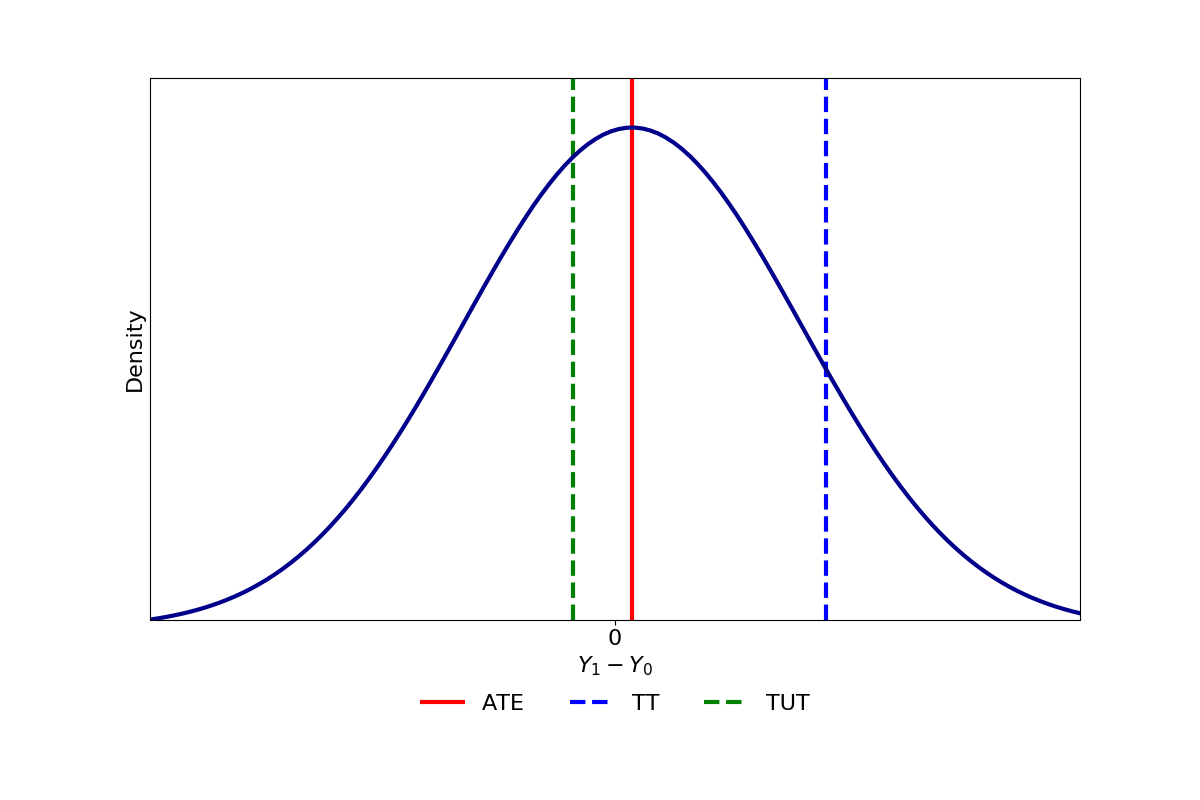
\includegraphics{fig-treatment-effects-with-eh}}
\end{figure}
\end{frame}

\begin{frame}
\begin{figure}\caption{Distribution of Effects without Essential Heterogeneity}
\scalebox{0.35}{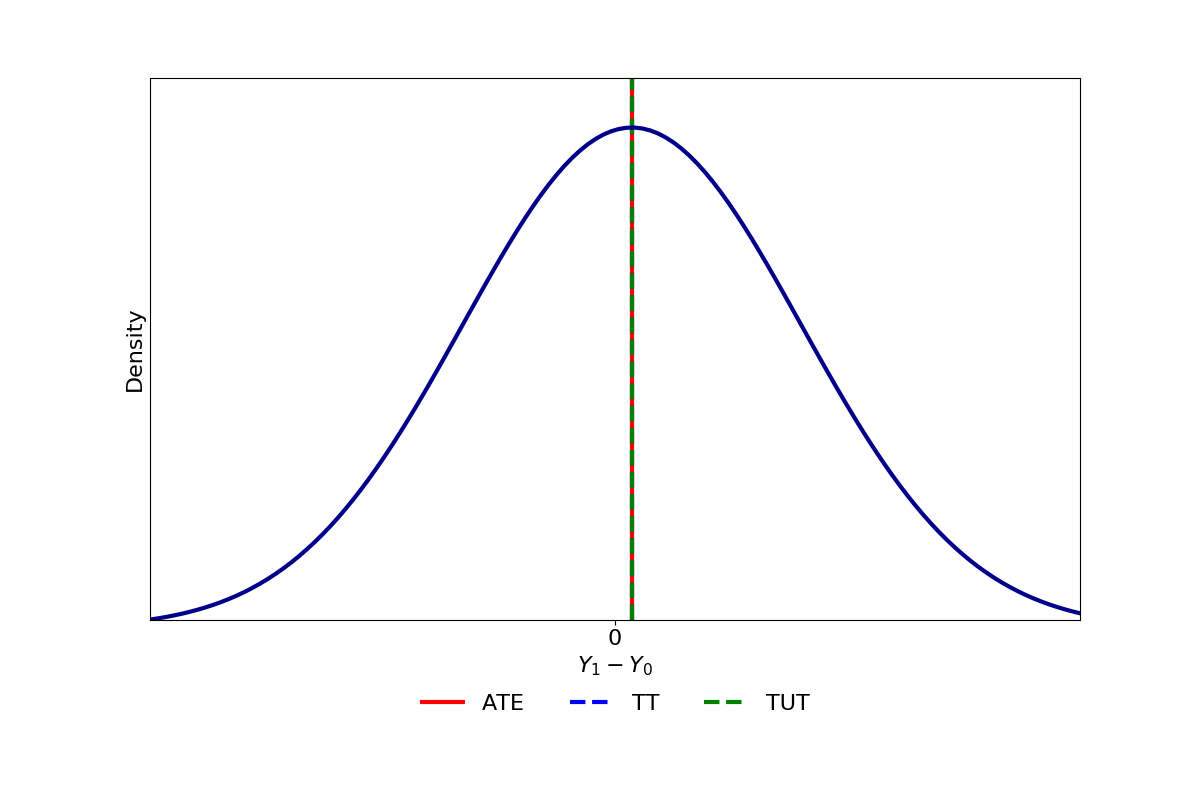
\includegraphics{fig-treatment-effects-without-eh}}
\end{figure}
\end{frame}

\begin{frame}
\begin{figure}\caption{Distribution of Benefits by Treatment Status}
\scalebox{0.35}{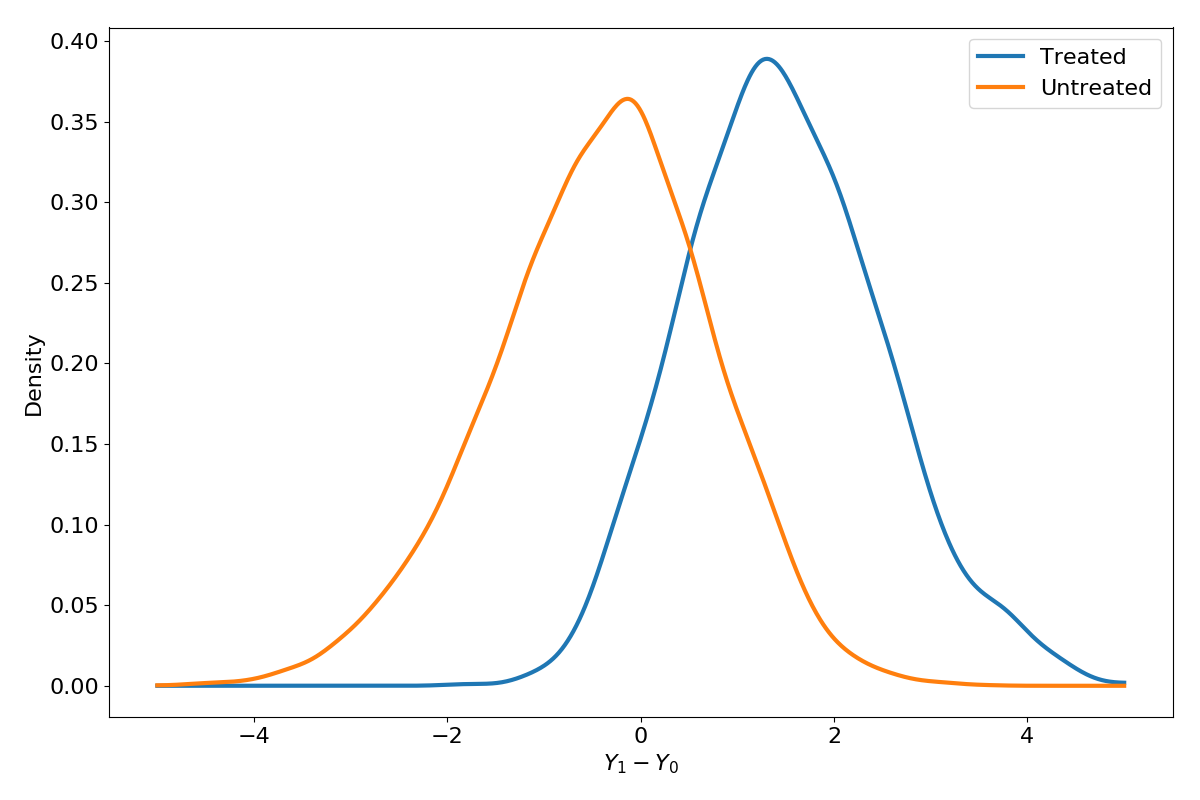
\includegraphics{fig-treatment-effects-treatment}}
\end{figure}
\end{frame}

%-------------------------------------------------------------------------------
%-------------------------------------------------------------------------------
\begin{frame}\begin{center}
\LARGE\textit{Policy-Relevant Average Treatment Effects}
\end{center}\end{frame}
%-------------------------------------------------------------------------------
%-------------------------------------------------------------------------------
\begin{frame}
\textbf{Observed Outcomes}

\begin{align*}
Y_B = D_B Y_1 + (1 - D_B) Y_0 \\
Y_A = D_A Y_1 + (1 - D_A) Y_0 \\
\end{align*}

\textbf{Effect of Policy}

\begin{align*}
B^{PRTE} = \frac{1}{E[D_A] - E[D_B]} (E[Y_A] - E[Y_B])
\end{align*}

\end{frame}


\begin{frame}
\begin{figure}\caption{Distribution of Benefits for Policy}
\scalebox{0.35}{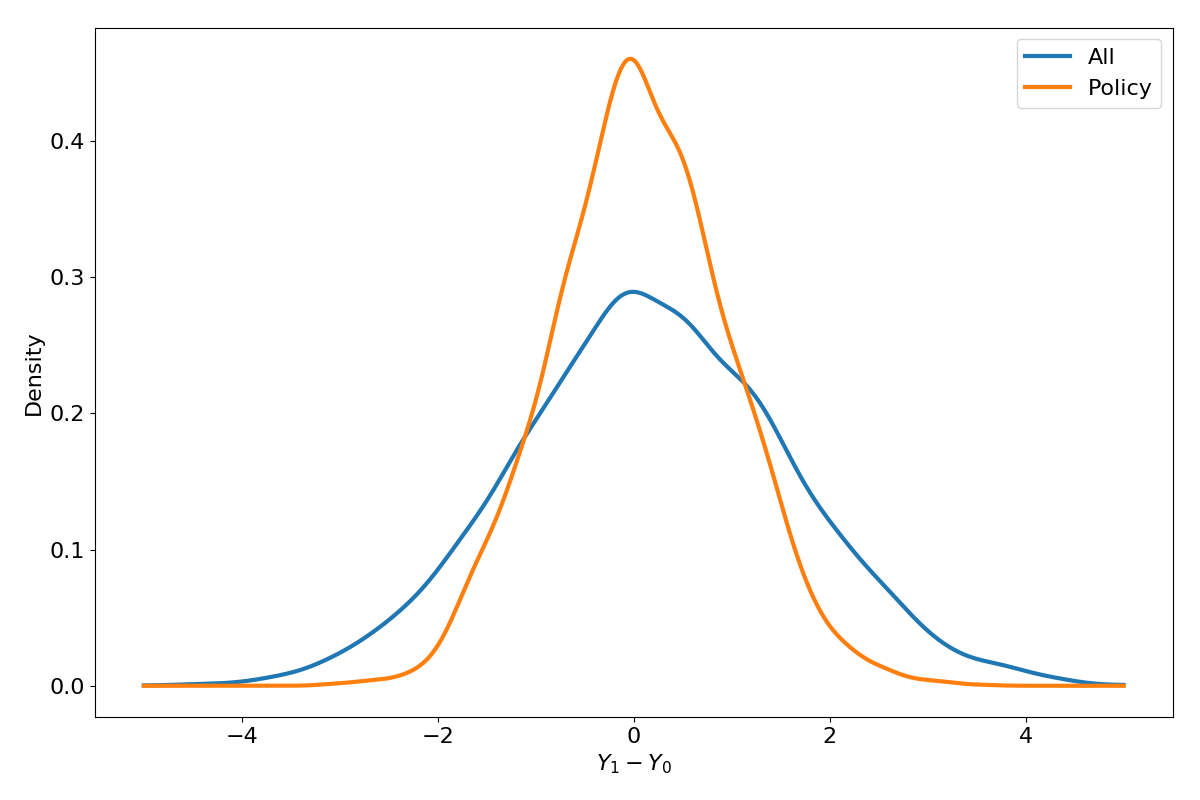
\includegraphics{fig-treatment-effects-policy}}
\end{figure}
\end{frame}

%-------------------------------------------------------------------------------
%-------------------------------------------------------------------------------
\begin{frame}\begin{center}
\LARGE\textit{Marginal Effect of Treatment}
\end{center}\end{frame}
%-------------------------------------------------------------------------------
%-------------------------------------------------------------------------------
\begin{frame}\textbf{Marginal Benefit of Treatment}

\begin{align*}
B^{MTE}(x, u_S) = E [Y_1 - Y_0 \mid X = x, U_S = u_S]
\end{align*}

\textbf{Intuition:} Mean gross return to treatment for persons at
quantile \(u_S\) of the first-stage unobservable \(V\).

\end{frame}

\begin{frame}
\begin{figure}\caption{Margin of Indifference}
\scalebox{0.35}{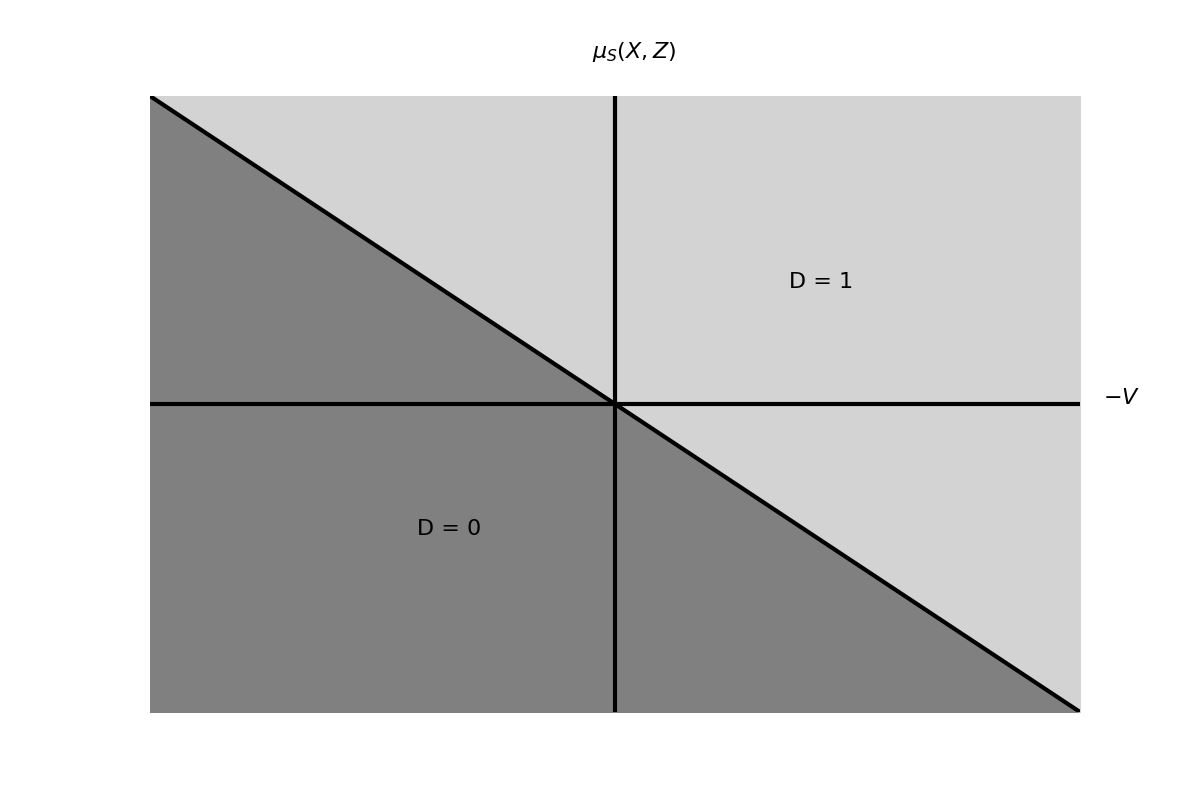
\includegraphics{fig-margin-indifference}}
\end{figure}
\end{frame}


\begin{frame}

\begin{figure}\caption{Marginal Effect of Heterogeneity}
\scalebox{0.35}{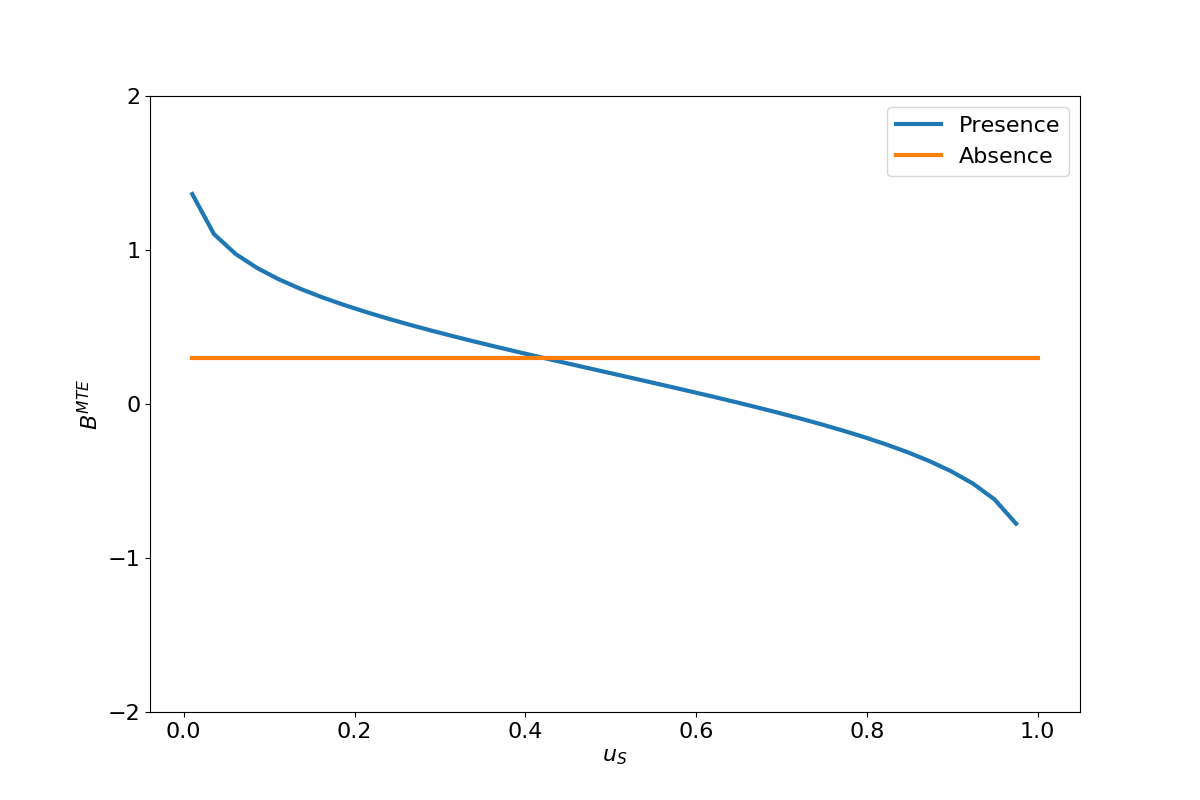
\includegraphics{fig-eh-marginal-effect}}
\end{figure}

\end{frame}


\begin{frame}
%\subsubsection{Effects of Treatment as Weighted Averages}\label{effects-of-treatment-as-weighted-averages}
\frametitle{Effects of Treatment as Weighted Averages}

Parameter \(\Delta_j\), can be written as a weighted average of the
\(B^{MTE}(x, u_S)\).

\begin{align*}
\Delta_j(x) = \int_0^1 B^{MTE}(x, u_S) \omega^j(x, u_S) du_S,
\end{align*}

where the weights \(\omega^j(x, u_S)\) are specific to parameter \(j\)
and integrate to one.
\end{frame}

\begin{frame}
\frametitle{Effects of Treatment as Weighted Averages}
\textbf{Weights}

\begin{align*}
 \omega^{ATE}(x, u_S) & = 1 \\
 \omega^{TT}(x, u_S) & = \frac{1 - F_{P\mid X=x}(u_S)}{E[P \mid X = x]}\\
 \omega^{TUT}(x, u_S) & = \frac{F_{P\mid X=x}(u_S)}{E[1 - P \mid X = x]}
\end{align*}

\end{frame}


\begin{frame}
\begin{figure}\caption{Effects of Treatment as Weighted Averages}
\scalebox{0.35}{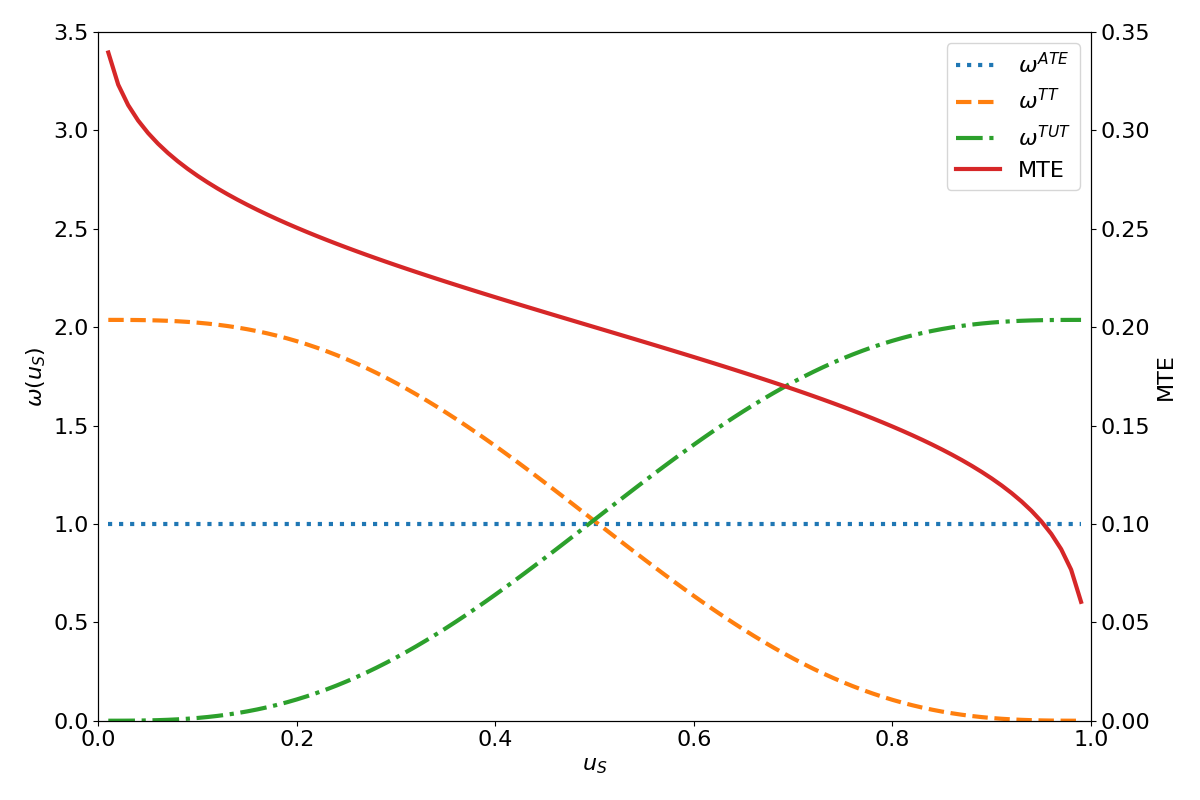
\includegraphics{fig-weights-marginal-effect.png}}
\end{figure}
\end{frame}

%-------------------------------------------------------------------------------
%-------------------------------------------------------------------------------
\begin{frame}\begin{center}
\LARGE\textit{Local Average Treatment Effect}
\end{center}\end{frame}
%-------------------------------------------------------------------------------
%-------------------------------------------------------------------------------
\begin{frame}
\textbf{Local Average Treatment Effect}

\begin{itemize}
\item \textbf{Local Average Treatment Effect:} Average effect for those induced
to change treatment because of a change in the instrument.
\(\Rightarrow\) instrument-dependet parameter

\item \textbf{Marginal Treatment Effect:} Average effect for those individuals
with a given unobserved desire to receive treatment.\\
\(\Rightarrow\) deep economic parameter
\end{itemize}
\end{frame}

\begin{frame}
    \begin{align*}
B^{LATE} = \frac{E(Y\mid Z = z) - E[Y \mid Z = z^\prime]}{P(z) - P(z^\prime)}
\end{align*}

\begin{align*}
B^{LATE}(x, u_S, u_{S^\prime}) = \frac{1}{u_S - u_{S^\prime}} \int_{u_S}^{u_{S^\prime}} B^{MTE}(x, u) du,
\end{align*}

\end{frame}


\begin{frame}
\begin{figure}[htp]\centering
	\caption{Local Average Treatment Effect}\label{Local Average Treatment}\scalebox{0.35}
	{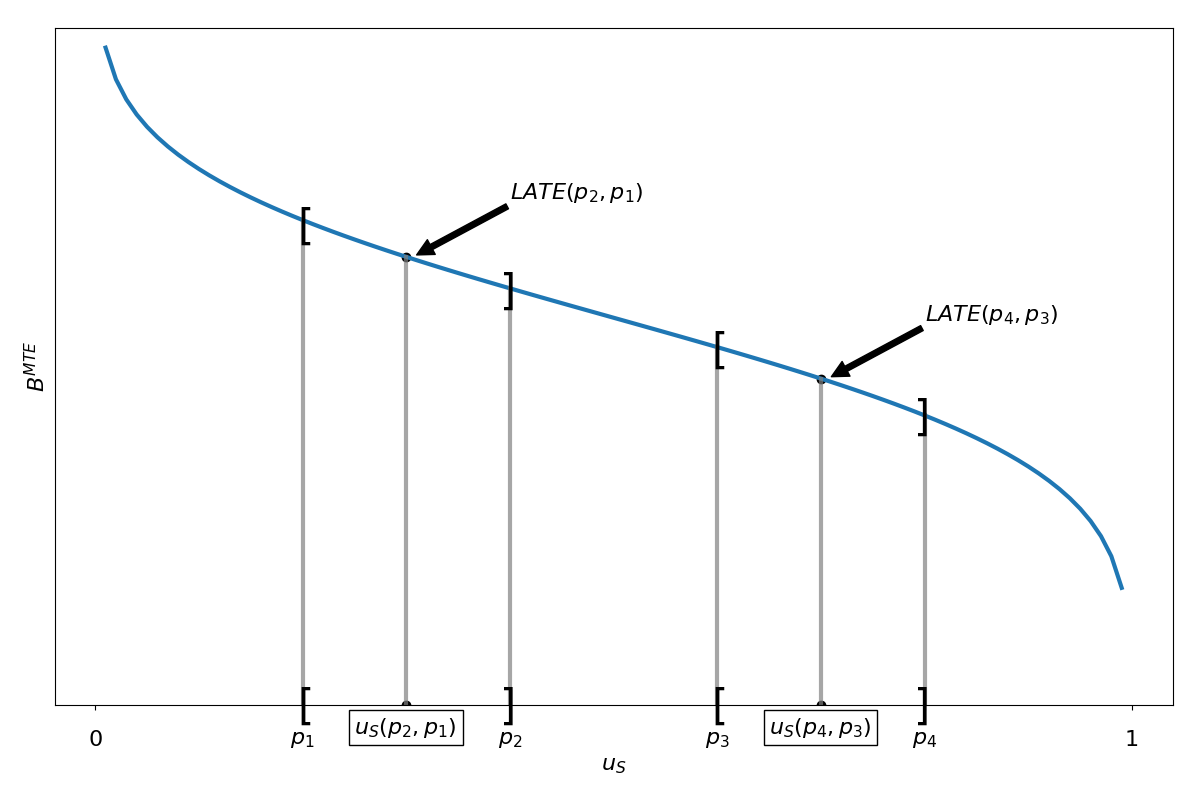
\includegraphics{fig-local-average-treatment.png}}
\end{figure}
\end{frame}

%-------------------------------------------------------------------------------
%-------------------------------------------------------------------------------
\begin{frame}\begin{center}
\LARGE\textit{Distributions of Effects}
\end{center}\end{frame}
%-------------------------------------------------------------------------------
%-------------------------------------------------------------------------------
\begin{frame}
\begin{figure}\caption{Distribution of Potential Outcomes}
\scalebox{0.35}{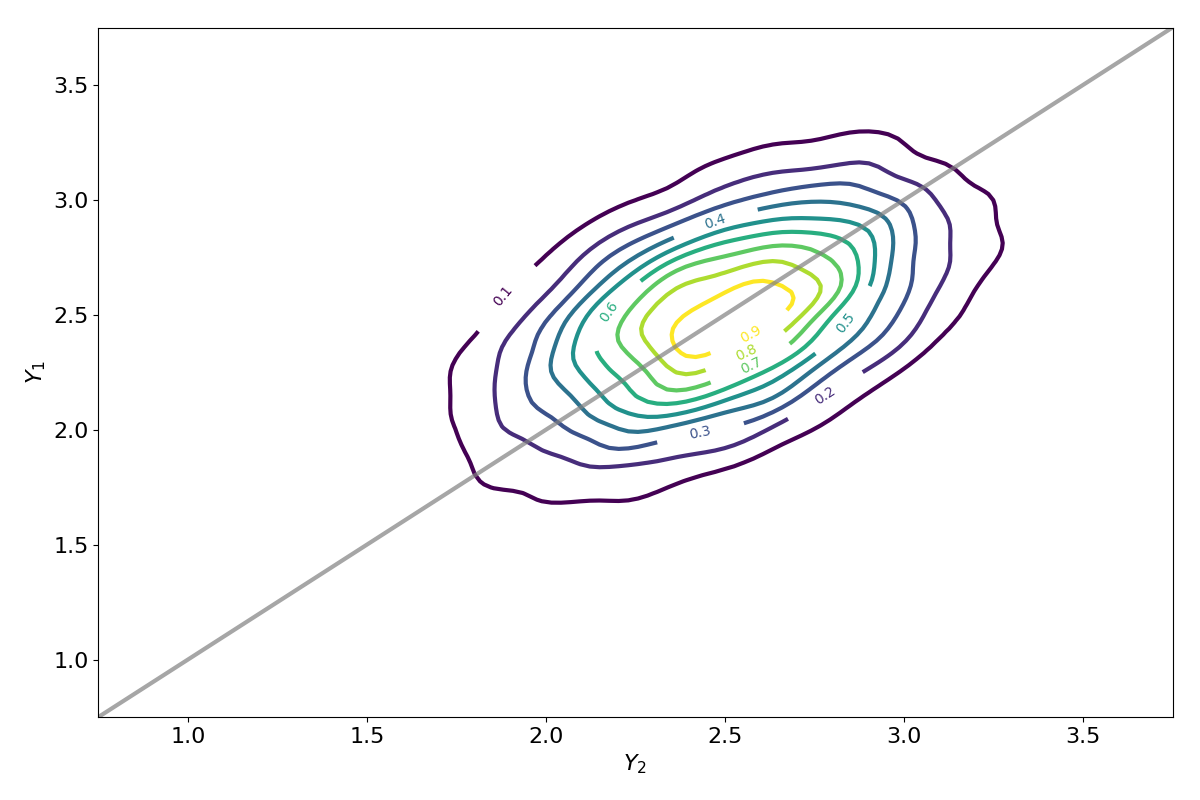
\includegraphics{fig-distribution-potential}}
\end{figure}
\end{frame}

\begin{frame}
\begin{figure}\caption{Distribution of Benefits and Surplus}
\scalebox{0.35}{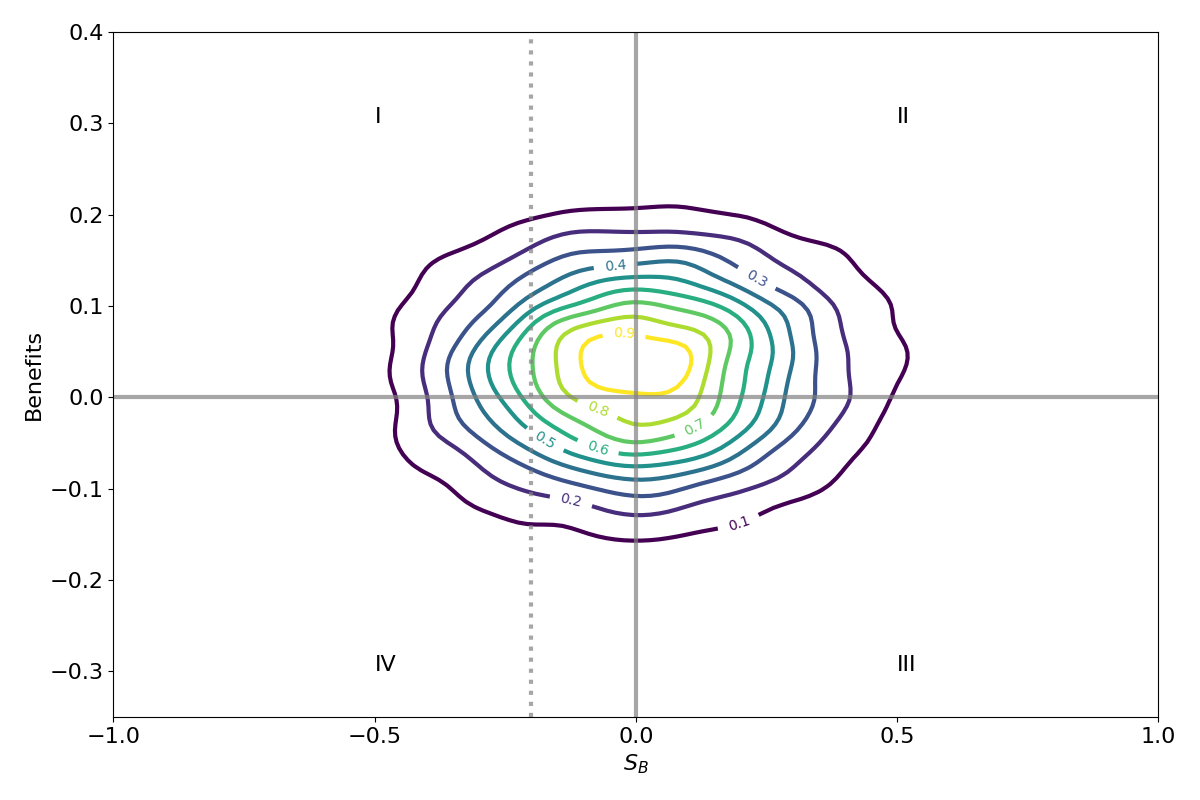
\includegraphics{fig-distribution-surplus}}
\end{figure}
\end{frame}


\beginbackup\appendix
\begin{frame}\begin{center}
\LARGE\textbf{Appendix}
\end{center}\end{frame}

%------------------------------------------------------------------------------
%------------------------------------------------------------------------------
\begin{frame}\begin{center}
\LARGE\textit{References}
\end{center}\end{frame}
%------------------------------------------------------------------------------
%------------------------------------------------------------------------------
\newgeometry{margin=1cm}
\begin{frame}[allowframebreaks]\frametitle{}

\nocite{Carneiro.2011, Heckman.1990c, Heckman.2010h}

\bibliographystyle{apalike}
\bibliography{../../../submodules/bibliography/literature}


\end{frame}

\backupend
\end{document}
